\documentclass[UTF8,a4paper,11pt,fontset=windows]{ctexart}

\usepackage{geometry}
\geometry{left=2.2cm,right=2.2cm,top=2.1cm,bottom=2.0cm}

\usepackage{xcolor}
\definecolor{Ink}{HTML}{1F2937}
\definecolor{Muted}{HTML}{5F6B7A}
\definecolor{Line}{HTML}{D9E2EF}
\definecolor{SoftBlue}{HTML}{EAF4FF}
\definecolor{DeepBlue}{HTML}{2454A6}
\definecolor{Violet}{HTML}{6D4AFF}
\definecolor{SoftViolet}{HTML}{F2EDFF}
\definecolor{SoftGreen}{HTML}{EAF8F0}
\definecolor{Warm}{HTML}{FFF5E8}
\definecolor{Night}{HTML}{080B1E}
\definecolor{Panel}{HTML}{151B3D}
\definecolor{NeonCyan}{HTML}{28E8FF}
\definecolor{NeonPurple}{HTML}{8E5CFF}
\definecolor{CoverCream}{HTML}{FFF8EC}

\usepackage{hyperref}
\hypersetup{
  colorlinks=true,
  linkcolor=DeepBlue,
  urlcolor=DeepBlue,
  citecolor=DeepBlue,
  pdfauthor={臧真宇},
  pdftitle={CanCan Campus Radio 产品说明文档}
}

\usepackage{graphicx}
\graphicspath{{assets/}{screenshots/}{PDF/assets/}{PDF/screenshots/}{../public/avatar/source/}{public/avatar/source/}}
\usepackage{array}
\usepackage{tabularx}
\usepackage{booktabs}
\usepackage{longtable}
\usepackage{enumitem}
\usepackage{tikz}
\usetikzlibrary{arrows.meta,positioning,shapes.geometric,calc}
\usepackage{caption}
\usepackage{float}
\usepackage{fancyhdr}
\usepackage{titlesec}
\usepackage{lastpage}
\usepackage{needspace}

\setlength{\parindent}{0em}
\setlength{\parskip}{0.45em}
\setlist[itemize]{leftmargin=1.5em,itemsep=0.12em,topsep=0.15em}
\setlist[enumerate]{leftmargin=1.7em,itemsep=0.12em,topsep=0.15em}
\renewcommand{\arraystretch}{1.22}
\captionsetup{font=small,labelfont=bf}
\sloppy

\pagestyle{fancy}
\fancyhf{}
\lhead{\small CanCan Campus Radio}
\rhead{\small 腾讯 PCG 校园 AI 产品创意大赛}
\cfoot{\small \thepage}
\renewcommand{\headrulewidth}{0.4pt}

\titleformat{\section}
  {\Large\bfseries\color{DeepBlue}}
  {\thesection}{0.8em}{}
\titleformat{\subsection}
  {\large\bfseries\color{Ink}}
  {\thesubsection}{0.75em}{}
\titleformat{\subsubsection}
  {\normalsize\bfseries\color{Ink}}
  {\thesubsubsection}{0.6em}{}

\newcommand{\pill}[1]{%
  \tikz[baseline=(X.base)] \node[draw=Line,fill=SoftBlue,rounded corners=8pt,inner xsep=8pt,inner ysep=3pt,font=\small\bfseries\color{DeepBlue}] (X) {#1};%
}

\newcommand{\callout}[2]{%
  \noindent
  \begin{tikzpicture}
    \node[
      fill=#1,
      draw=Line,
      rounded corners=5pt,
      inner sep=10pt,
      text width=\dimexpr\linewidth-22pt\relax,
      align=left
    ] {#2};
  \end{tikzpicture}
}

\newcommand{\infobox}[2]{%
  \noindent
  \begin{tikzpicture}
    \node[
      fill=#1,
      draw=Line,
      rounded corners=6pt,
      inner sep=12pt,
      text width=\dimexpr\linewidth-26pt\relax,
      align=left
    ] {#2};
  \end{tikzpicture}
}

\newcommand{\placeholder}[3]{%
  \begin{figure}[H]
    \centering
    \begin{tikzpicture}
      \draw[rounded corners=4pt,draw=Line,fill=SoftBlue] (0,0) rectangle (14.2,5.4);
      \draw[rounded corners=3pt,draw=DeepBlue!35,fill=white] (0.6,0.4) rectangle (13.6,5.0);
      \draw[draw=Line,fill=SoftViolet] (0.6,4.45) rectangle (13.6,5.0);
      \foreach \x in {1.0,1.4,1.8} {
        \fill[DeepBlue!45] (\x,4.72) circle (0.07);
      }
      \node[align=center,text width=11.8cm,color=Ink,font=\bfseries] at (7.1,2.9) {#1};
      \node[align=center,text width=11.8cm,color=Muted,font=\small] at (7.1,2.1) {产品界面截图预留位：\texttt{PDF/screenshots/#2}};
      \node[align=center,text width=11.8cm,color=Muted,font=\small] at (7.1,1.3) {#3};
    \end{tikzpicture}
    \caption{#1}
  \end{figure}
}

\newcommand{\screenshotfigure}[3]{%
  \begin{figure}[H]
    \centering
    \includegraphics[width=#3\linewidth,keepaspectratio]{#2}
    \caption{#1}
  \end{figure}
}

% ---------- 文档正文 ----------
\begin{document}

% ========== 封面 ==========
\begin{titlepage}
  \thispagestyle{empty}
  \begin{tikzpicture}[remember picture,overlay]
    \fill[white] (current page.south west) rectangle (current page.north east);
    \shade[left color=Night,right color=Panel] (current page.north west) rectangle ($(current page.north east)+(0,-16.8cm)$);
    \fill[CoverCream] ($(current page.south west)+(0,0)$) rectangle ($(current page.south east)+(0,5.2cm)$);
    \fill[NeonPurple!16] ($(current page.south west)+(0,0)$) rectangle ($(current page.south east)+(0,1.25cm)$);
    \draw[NeonCyan,line width=0.9pt] ($(current page.north west)+(1.7cm,-16.8cm)$) -- ($(current page.north east)+(-1.7cm,-16.8cm)$);

    \foreach \x/\h in {1.6/0.35,1.95/0.7,2.3/0.45,2.65/1.05,3.0/0.55,3.35/0.85,3.7/0.42,4.05/0.65} {
      \fill[NeonCyan!45] ($(current page.north west)+(\x cm,-14.55cm)$) rectangle ++(0.13cm,\h cm);
    }
    \foreach \x/\h in {16.8/0.5,17.15/0.9,17.5/0.6,17.85/1.15,18.2/0.78,18.55/0.48,18.9/0.92} {
      \fill[NeonPurple!55] ($(current page.north west)+(\x cm,-14.55cm)$) rectangle ++(0.13cm,\h cm);
    }
    \foreach \x/\y in {5.7/-1.45,9.3/-2.1,16.0/-1.7,18.2/-5.3,3.5/-10.6} {
      \fill[NeonCyan!60] ($(current page.north west)+(\x cm,\y cm)$) rectangle ++(0.08cm,0.08cm);
      \fill[NeonPurple!75] ($(current page.north west)+(\x cm+0.12cm,\y cm+0.12cm)$) rectangle ++(0.08cm,0.08cm);
    }

    \node[anchor=north west,text=NeonCyan,font=\large\bfseries] at ($(current page.north west)+(2.0cm,-1.75cm)$)
      {腾讯 PCG 校园 AI 产品创意大赛 · 开放赛道};
    \node[anchor=north west,align=left,text=white,font=\bfseries] at ($(current page.north west)+(2.0cm,-2.85cm)$)
      {\fontsize{31}{37}\selectfont CanCan\\[-0.05cm]Campus Radio};
    \node[anchor=north west,text=NeonCyan!92,font=\Large] at ($(current page.north west)+(2.05cm,-5.65cm)$)
      {大学生的 AI 情绪陪伴电台};
    \node[anchor=north west,draw=NeonCyan!42,fill=Panel,rounded corners=8pt,inner sep=12pt,text width=8.0cm,align=left,text=white,font=\small] at ($(current page.north west)+(2.0cm,-6.65cm)$)
      {\textbf{\color{NeonCyan}一句话概述：}CanCan Campus Radio 面向校园生活中需要慢下来、重新整理心情的大学生。它让 AI DJ 灿灿理解用户当下的状态，用合适的歌曲、温柔的口播和可持续记忆，陪学生度过早八、图书馆、考试周、深夜 Deadline 和独处发呆的时刻。};

    \node[anchor=north west,draw=NeonPurple!62,line width=0.9pt,fill=Night,rounded corners=10pt,inner sep=5pt] at ($(current page.north west)+(11.45cm,-1.82cm)$)
      {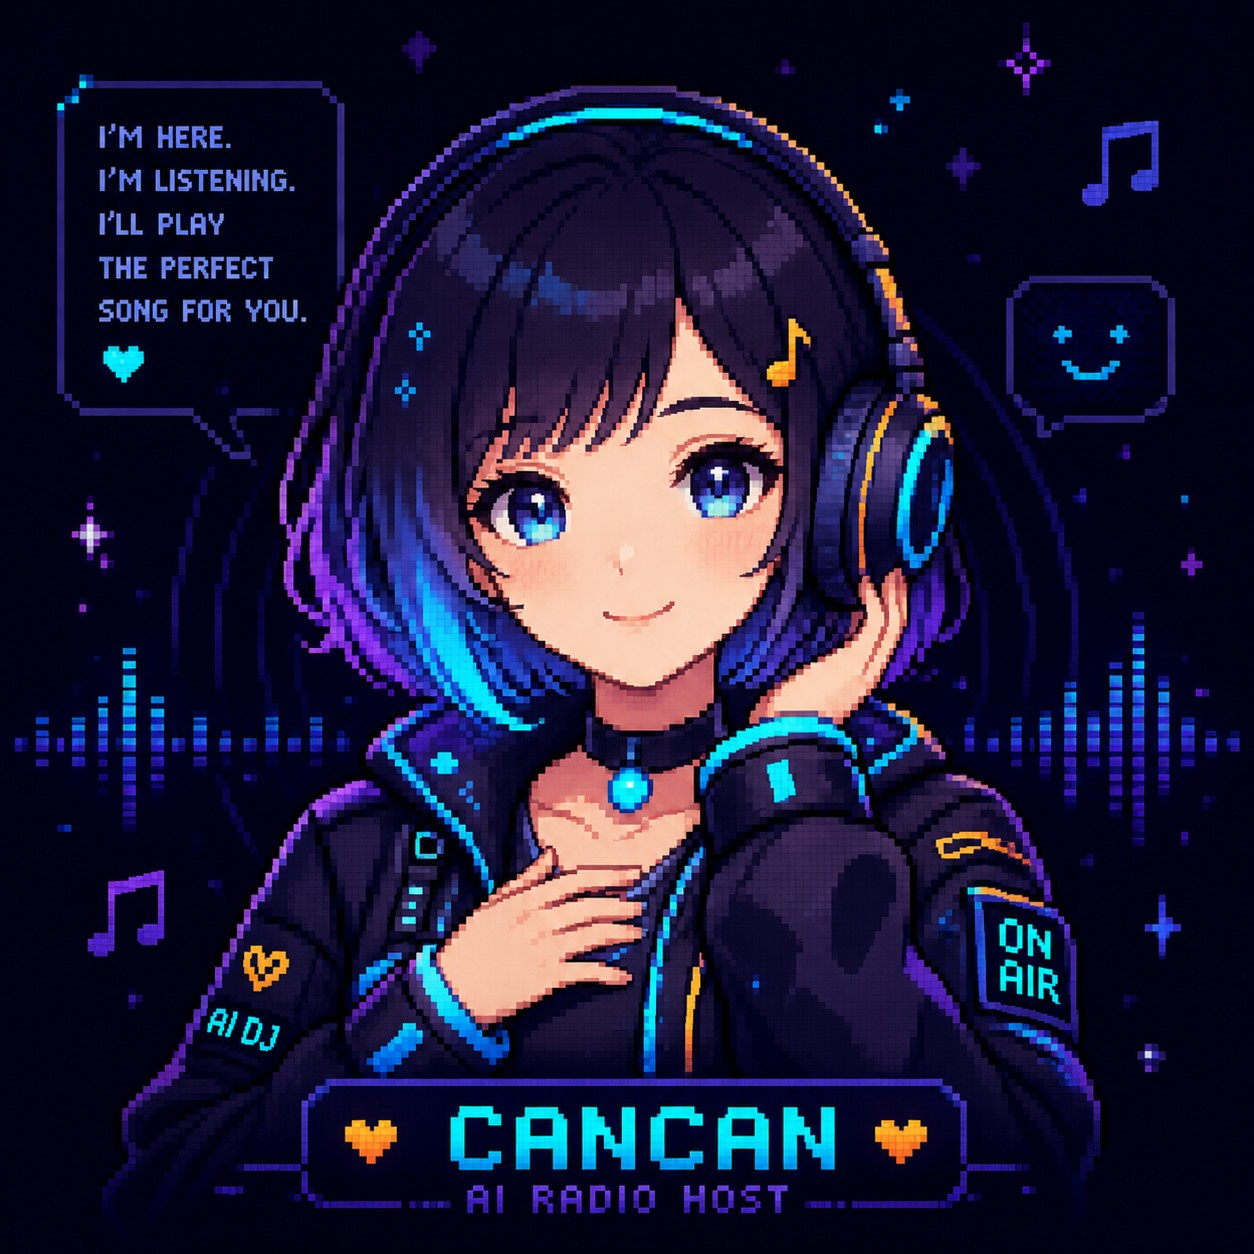
\includegraphics[width=7.0cm]{cancan-cover.jpg}};
    \node[anchor=north west,draw=NeonCyan!55,fill=Night,rounded corners=12pt,inner xsep=12pt,inner ysep=5pt,text=NeonCyan,font=\bfseries] at ($(current page.north west)+(12.45cm,-9.28cm)$)
      {灿灿 · AI RADIO HOST};
    \node[anchor=north west,text=NeonPurple!82,font=\small] at ($(current page.north west)+(12.45cm,-10.05cm)$)
      {会聊天、会推荐、会记住反馈的虚拟电台主持人};

    \node[anchor=north west,fill=white,draw=Line,rounded corners=8pt,inner sep=14pt,text width=15.9cm,align=left] at ($(current page.north west)+(2.5cm,-17.7cm)$)
      {
        {\large\bfseries\color{DeepBlue} 作品信息}\par
        \vspace{0.35cm}
        \begin{tabularx}{15.3cm}{>{\raggedleft\arraybackslash\bfseries\color{Muted}}p{3.1cm} >{\raggedright\arraybackslash}X}
          作品名称 & \textbf{CanCan Campus Radio} \\[0.38em]
          参赛赛道 & 开放赛道 \\[0.38em]
          选手姓名 & 臧真宇 \\[0.38em]
          Demo 链接 & \href{http://114.132.166.178}{腾讯云公网 Demo：http://114.132.166.178}；本地 Windows Release 备用包作为备用体验 \\[0.38em]
          提交材料 & 产品说明文档 PDF \\
        \end{tabularx}

        \vspace{0.5cm}
        {\large\bfseries\color{DeepBlue} 体验提示}\par
        \vspace{0.3cm}
        \begin{tabularx}{15.3cm}{>{\raggedleft\arraybackslash\bfseries\color{Muted}}p{3.1cm} >{\raggedright\arraybackslash}X}
          浏览器 & 建议使用 \textbf{Chrome 浏览器}访问，以获得最佳音频播放体验 \\[0.38em]
          快速体验 & 进入页面后\textbf{无需登录}，可直接点击「\textbf{启动电台}」体验完整流程 \\[0.38em]
          推荐输入 & 试试输入：「\textbf{我在图书馆有点焦虑，想开始复习}」 \\
        \end{tabularx}
      };
    \node[anchor=south,align=center] at ($(current page.south)+(0,1.65cm)$)
      {\pill{AI 电台}\quad \pill{校园情绪陪伴}\quad \pill{音乐推荐}\quad \pill{调音台控制台}\quad \pill{腾讯云 Demo}};
  \end{tikzpicture}
\end{titlepage}

\setcounter{page}{2}

\setcounter{tocdepth}{1}
\tableofcontents
\newpage

% ========== Demo 入口提醒 ==========
\callout{SoftBlue}{\textbf{\color{DeepBlue}Demo 入口：}当前公开 Demo 已部署在腾讯云，访问 \href{http://114.132.166.178}{http://114.132.166.178}。建议使用 Chrome 浏览器，无需登录即可体验完整流程。推荐输入：「我在图书馆有点焦虑，想开始复习。」线上版本使用参赛者本人网易云账号作为测试曲库，每位访客的聊天、偏好、反馈和记忆进入独立沙盒，互不影响。}

% ========== 一分钟看懂 CanCan ==========
\section{一分钟看懂 CanCan}

\begin{longtable}{>{\bfseries}p{3.2cm}p{11.4cm}}
\toprule
维度 & 一句话 \\
\midrule
一句话定位 & 面向大学生的 AI 情绪陪伴电台：用户说状态，AI DJ 用音乐和口播陪学生度过校园生活的真实时刻。 \\
目标用户 & 在早八、图书馆、考试周、深夜 Deadline 和独处时刻需要音乐陪伴的大学生。 \\
核心痛点 & 不是没歌可听，而是在疲惫、焦虑、专注切换时，缺少一个能理解当下状态、降低选歌成本、保持低打扰陪伴的声音入口。 \\
核心方案 & 用户说状态 → AI 理解 → 灿灿推荐歌曲并用口播解释 → 用户边听边反馈 → 系统记住偏好。每一次用完，下一次就更懂你。 \\
AI 能力 & AI 不只是负责回答几句话，而是决定这段电台怎么继续：用户说了什么、现在适合什么歌、灿灿要不要开口、哪些反馈下次要记住、要不要生成一段原创声音。 \\
Demo 入口 & \href{http://114.132.166.178}{http://114.132.166.178}（腾讯云公网，Chrome 浏览器，无需登录） \\
PCG 价值 & 它不是又一个播放器，而是把音乐、播客、OST 和校园内容整理成一段可以听的时间。对 PCG 来说，它更像一个低打扰的校园内容入口。 \\
\bottomrule
\end{longtable}

% ========== Demo 推荐体验流程 ==========
\section{Demo 推荐体验流程}

建议评委按这个顺序体验，5 分钟内可以跑完整个核心流程。

\begin{longtable}{>{\bfseries}p{0.6cm}p{4.7cm}p{9.3cm}}
\toprule
\# & 操作 & 评委能看到什么 \\
\midrule
1 & 打开公网 Demo \href{http://114.132.166.178}{114.132.166.178} & 进入 CanCan 电台主界面，看到 AI DJ 灿灿头像、播放器区域、调音台入口和启动电台按钮。无需登录，无需配置。 \\
2 & 点击「启动电台」 & 灿灿头像从静止变为 on air 状态，系统创建会话 Session，根据曲库画像和当前时间天气生成第一段 TTS 语音口播并推荐第一首歌。 \\
3 & 输入「我在图书馆有点焦虑，想开始复习」 & 灿灿理解状态后生成针对性口播，歌曲推荐风格偏向低打扰、稳定节奏的背景音乐，推荐依据标签展示（如「聊天语境」「曲库画像」「天气时间」）。 \\
4 & 点击「不喜欢」或输入「这首太吵了」 & 灿灿根据反馈调整推荐方向，降低节奏强度或切换曲风，并在后续口播中体现出已收到反馈。这验证了反馈对体验的即时影响。 \\
5 & 打开调音台 & 看到聊天/推歌比例滑块、主动推荐频率、语音播报开关、情绪模式、低打扰模式和记忆管理面板。调整低打扰模式后返回主界面，口播频率和推荐节奏明显变化。 \\
6 & 打开 AI 原创电台模式 & 灿灿调用 AI 音乐生成能力创建原创声音片段，适用于版权受限或需要专属校园声音的场景。这是对既有曲库推荐的补充。 \\
\bottomrule
\end{longtable}

% ========== 项目故事：写在前面 ==========
\section{项目故事：为什么校园需要一个安静的 AI 电台}

做这个产品之前，我经常有一种很具体的感受：一天已经很累了，回到宿舍想放松一下，却还是下意识打开短视频。原只想看五分钟，结果半小时过去，屏幕一直很热闹，人却没有真的休息下来。

校园生活里有很多这样的时刻。早八路上困得睁不开眼，图书馆坐下后迟迟进不了状态，考试周夜里明明焦虑却还要继续写，宿舍熄灯后戴着耳机，想找点声音陪着自己。我们不是没有内容可以看，也不是没有歌可以听，而是经常缺少一个能把人从嘈杂里轻轻拉出来的地方。

音乐原本就有这种力量。它不要求我一直盯着屏幕，也不要求我立刻说清楚自己怎么了。一首刚好合适的歌，有时候比很多安慰都更有效。但问题是，当音乐产品也越来越像信息流——用户在歌单、榜单、推荐和搜索之间继续选择——想听歌的人，最后又变成了一个需要不断做决定的人。

CanCan Campus Radio 想做的就是把这件事变轻。核心思路不是再做一个播放器，也不是给播放器套一个 AI 聊天框。而是让「状态表达」成为听歌的入口：用户说一句「今天有点烦，想安静一会儿」，AI DJ 灿灿就理解此刻状态，从用户自己的音乐偏好里找一首合适的歌，用几句不打扰的口播递过来。它不想让学生打开之后又进入新的信息流，而是希望那几分钟像一个可以呼吸的房间。

\textbf{大学生不是没有内容或音乐，而是缺少低打扰、能理解当下状态的声音入口。}这句话是理解 CanCan 价值的主线。

% ========== 用户洞察与问题定义 ==========
\section{用户洞察与问题定义}

\subsection{目标用户}

只要是喜欢音乐的大学生，都是 CanCan 想服务的人。赶早八的路上、图书馆里复习、社团活动结束后的空档、深夜在宿舍戴着耳机——在这些时刻，音乐本来就该是一件简单的事：不用选、不用搜、不用做决定，只需要一个能听懂你状态的声音陪着。

\begin{longtable}{>{\bfseries}p{3.2cm}p{11.4cm}}
\toprule
用户类型 & 典型特征 \\
\midrule
高压学习型学生 & 课程、实验、考试、论文和实习申请叠在一起，经常需要在短时间内切换状态。听歌不是为了热闹，而是为了进入专注、缓和焦虑或撑过疲惫。 \\
情绪敏感型学生 & 容易被人际关系、成绩反馈、未来不确定性影响心情。有表达欲，但不一定想把每次低落都发到社交平台。 \\
独处陪伴型学生 & 宿舍、通勤、夜跑或深夜自习时经常一个人听歌，希望有人「在场」，但不希望被过度打扰。 \\
音乐收藏型学生 & 平时有自己的歌单、收藏和偏好，希望 AI 不是凭空推荐热门歌，而是理解自己的音乐历史。 \\
\bottomrule
\end{longtable}

\subsection{用户痛点与典型场景}

\textbf{大学生不是没有音乐可以听，而是在疲惫、焦虑、专注切换等场景中，缺少一个能理解当下状态、降低选歌成本、保持低打扰陪伴的音乐入口。}

\subsubsection{痛点一：学生想用音乐调节状态，但「选歌」本身也有成本}

很多学生打开音乐软件时，并不是为了认真探索新歌，而是想把自己从某种状态里带出来：困、烦、焦虑、分心、空落落。但真正开始听之前，还要搜索、翻歌单、判断风格、切掉不合适的歌。人在疲惫的时候，连选一首合适的歌都会变成额外负担。

\subsubsection{痛点二：音乐推荐知道「我爱听什么」，但不一定知道「我现在怎么了」}

传统音乐推荐更擅长根据历史播放、收藏、相似歌曲推测偏好。这对「找好听的歌」有帮助，但对校园场景里的即时语境并不够。早八的困、考试前的焦虑、论文卡住的烦、失眠时的不安——这些状态不是一个固定歌单能长期解决的。用户需要的是「此刻适合我」的音乐，而不是单纯「我可能喜欢」的音乐。

\subsubsection{痛点三：普通播放器只会播放，AI 聊天又很难进入听歌流程}

普通播放器只负责「播什么」，不会解释为什么这首歌适合现在，也不会记住用户刚说过「别太吵」。而很多 AI 聊天产品虽然能对话，却没有真正进入听歌流程，容易变成「聊天机器人旁边放了个播放器」。CanCan 要解决的不是聊天本身，而是把聊天、推荐、口播、播放和反馈串成一个连续流程。

\subsubsection{使用场景}

\begin{longtable}{>{\bfseries}p{2.8cm}p{5.4cm}p{6.4cm}}
\toprule
场景 & 用户状态 & 产品回应 \\
\midrule
早八通勤 & 没睡醒，路上需要一点清醒感，但不想被强节奏轰炸。 & AI DJ 选择轻快但不过度兴奋的歌曲，用短口播帮助用户进入一天。 \\
图书馆专注 & 想进入学习状态，怕歌词和短视频打断注意力。 & 推荐更适合背景陪伴的音乐，减少口播密度，保持低打扰。 \\
考试周焦虑 & 心里很乱，想找一点稳定感。 & 先回应压力存在，再用舒缓歌曲和温柔口播帮用户降速。 \\
熬夜 Deadline & 疲惫但还要继续完成任务。 & 推荐节奏稳定、能支撑行动的歌曲，口播更像陪跑而不是说教。 \\
宿舍放松 & 一天结束后想从社交和学习里退出来。 & 生成一个更像私人夜间电台的播放体验，让用户慢慢收尾。 \\
\bottomrule
\end{longtable}

% ========== 典型用户一天的故事 ==========
\subsection{典型用户一天的故事}

下面是一个普通大学生的一天——CanCan 在每个时刻能做什么。

\begin{longtable}{>{\bfseries}p{1.8cm}p{2.4cm}p{4.2cm}p{5.2cm}}
\toprule
时间 & 场景 & 状态 & CanCan 的回应 \\
\midrule
早上 8:00 & 早八通勤 & 困、没精神、不想被强节奏轰炸 & 轻快但不过度兴奋的歌曲搭配简短开场口播，帮用户慢慢醒来而不制造压力。 \\
下午 2:00 & 图书馆 & 想专注但有点焦虑 & 低打扰歌单，减少口播频率和长度，让音乐成为背景陪伴而不是注意力干扰。 \\
晚上 9:30 & Deadline 前 & 累但还要继续写 & 稳定节奏的歌曲搭配陪跑式口播，不喊加油也不说教，只是让人感觉「有人在旁边」。 \\
深夜 0:30 & 宿舍 & 不想刷短视频但睡不着 & 温柔的夜间电台模式，降低亮度、放慢节奏、减少语言密度，帮助用户从一天中慢慢退出来。 \\
\bottomrule
\end{longtable}

% ========== 旧体验 vs CanCan ==========
\subsection{旧体验 vs CanCan 体验}



\begin{longtable}{>{\bfseries}p{2.5cm}p{4.0cm}p{4.0cm}p{4.1cm}}
\toprule
维度 & 普通音乐软件 & 普通 AI 聊天 & CanCan Campus Radio \\
\midrule
入口 & 搜索 / 歌单 / 榜单 / 推荐流 & 文字对话框 & 状态表达：说一句「今天有点烦」即可启动电台 \\
推荐逻辑 & 历史播放 + 相似歌曲 + 热门趋势 & 无音乐推荐能力，或作为附加功能 & 聊天语境 + 曲库画像 + 反馈记忆 + 时间天气 + 可播放性 \\
陪伴方式 & 没有陪伴，只负责播放 & 可以聊天，但脱离音乐播放流程 & AI DJ 口播 + TTS 语音 + 头像状态 + 歌曲推荐形成完整陪伴 \\
反馈影响 & 喜欢 / 不喜欢影响后续推荐（延迟） & 对话级别反馈，不沉淀为音乐偏好 & 实时反馈影响当前和下一轮推荐，长期记忆持续优化 \\
用户控制 & 播放器控制（播放/暂停/切歌） & 对话控制（聊什么 / 不聊什么） & 调音台控制（聊天/推歌比例、低打扰、情绪模式、记忆管理） \\
核心体验 & 听歌 & 聊天 & 聊天 + 推荐 + 播放 + 口播 + 反馈 + 记忆 → 越听越懂你的电台 \\
\bottomrule
\end{longtable}

% ========== 产品方案设计 ==========
\section{产品方案设计}

\subsection{产品概述}

\textbf{CanCan 把「聊天」和「听歌」组织成同一个流程：AI DJ 理解状态 → 从曲库里找到合适的歌 → 用口播解释为什么选这首 → 播放中接收反馈 → 记住偏好，下次推荐更准。}

用户打开 CanCan，可以用自然语言告诉它现在的状态——「我在图书馆有点焦虑，想开始复习」——也可以直接点自习室、教室这些校园场景入口。灿灿会结合用户的音乐偏好、曲库画像、近期反馈、时间天气和聊天语境，生成一段电台式回应，然后把一首歌接进来。

在这个过程中，用户不是面对一个歌单再做选择题，也不是和一个聊天机器人闲聊。聊天、推荐、口播、播放、反馈是同一个流程里的不同环节：说「这首太吵了」，下一首就放轻；说「现在不想被安慰」，口播就变少、歌更稳。灿灿的对话和口播由 DeepSeek V4 支撑，语音合成接的是火山引擎豆包 TTS，AI 原创模式接的是 MiniMax。

CanCan 希望做到的其实就三件事：让用户能把模糊的状态说出来，不用学什么 prompt；让每首歌都有个简短的理由，不是随机蹦出来的；让反馈和记忆留下来，下次打开电台的时候，灿灿比上次更知道分寸。

\screenshotfigure{产品主界面：用户可以在同一界面完成听歌、聊天、查看推荐依据和进入调音台。}{01-home.png}{0.98}

% ========== CanCan 的 4 个核心创新 ==========
\subsection{CanCan 的 4 个核心创新}

CanCan 用到的技术——LLM 对话、TTS 语音合成、音乐推荐、虚拟头像——单独看都不新。它的价值不在单点技术，而在于把这些能力装进一个具体的校园听歌场景里，让学生从「又要选歌、又要刷屏」的循环里走出来。

\begin{enumerate}
  \item \textbf{不只是给歌单，而是接一段电台。}传统推荐直接给结果列表，CanCan 先生成一段贴合场景的 DJ 口播，展示推荐依据标签，让用户知道这首歌为什么适合现在，然后才进入播放。它不是推荐引擎加了一个语音播报，而是把推荐重新设计为「电台主持人接歌」的体验。
  \item \textbf{不只看长期偏好，也看用户此刻怎么了。}大多数推荐系统依赖历史数据判断「你爱听什么」，但校园生活里，「此刻状态」和「长期偏好」同等重要。CanCan 把聊天语境（我刚说了什么）、时间天气（现在是深夜还是早八）、反馈趋势（最近频繁跳过什么）同时纳入推荐决策，让推荐从「你喜欢的歌」变成「此刻适合你的歌」。
  \item \textbf{不把聊天和播放拆开，而是让它们互相影响。}很多 AI 聊天产品把音乐当作附加功能（聊完发一首歌），而 CanCan 的聊天和播放是同一个流程：用户一边听歌一边聊天，聊天内容实时影响推荐和口播，播放反馈反过来影响后续对话策略。聊天不是产品的外壳，而是推荐引擎的输入端。
  \item \textbf{不制造更多刺激，而是把注意力还给用户。}短视频、信息流和社交通知都在争夺注意力，但校园里有很多时刻——复习、通勤、睡前——学生需要的不是更多刺激，而是有声音在场但不抢注意力。CanCan 的低打扰模式、歌单模式和 TTS 口播设计，都是为了让用户可以不盯屏幕完成整个听歌体验。
\end{enumerate}

% ========== 核心功能（四大模块） ==========
\subsection{核心功能（四大模块）}

CanCan 的功能分成四个模块，每个模块解决电台体验的一个环节。

\begin{longtable}{>{\bfseries}p{2.3cm}>{\bfseries}p{2.8cm}p{9.5cm}}
\toprule
模块 & 能力 & 说明 \\
\midrule
\endfirsthead
\bottomrule
\endhead
AI DJ 电台 & 启动电台 & 用户进入主界面后可直接启动，系统创建会话 Session，读取偏好与候选歌曲，生成第一段 AI DJ 口播并推荐第一首歌。 \\
& 口播生成与 TTS 播报 & LLM 生成短句式、低打扰的电台主持文案，解释歌曲与此刻状态的关系。接入火山引擎豆包 TTS 将文案转为语音。 \\
& AI DJ 头像状态 & 头像随 searching、talking、listening、happy、on air 等状态变化，让产品从工具界面变成有主持人存在的电台空间。 \\
& 场景与情绪输入 & 用户可用自然语言描述状态，也可直接选择自习室、教室、健身房等校园场景入口。 \\
\midrule
个性化推荐 & 曲库画像 & 分析用户歌单、常听艺人、流派倾向、情绪标签和探索方向，用户可手动选择哪些歌单参与长期画像。 \\
& 场景识别与推荐 & 结合聊天语义、曲库画像、近期反馈、情绪模式、时间天气和可播放性，选择更合适的歌曲。 \\
& 推荐依据标签 & 每次推荐展示若干依据标签（聊天语境、天气时间、曲库画像、近期反馈），让推荐理由透明可见。 \\
& 歌单模式 & 灿灿可一次整理一组连续推荐后按队列播放，适合自习、通勤等不想盯着屏幕的场景。 \\
\midrule
反馈与记忆 & 喜欢/不喜欢/跳过 & 实时反馈影响当前推荐策略和口播风格，而非仅在后台异步更新。 \\
& 长期记忆 & 聊天偏好、播放反馈和补充说明沉淀为长期记忆，用户可在调音台中查看、编辑或删除。 \\
& 反馈趋势 & 追踪「最近频繁跳过什么」「什么时段喜欢哪种风格」等趋势，让推荐越来越贴合个人节奏。 \\
\midrule
用户控制 & 调音台 & \texttt{/mixer} 页面提供聊天/推歌比例、主动推荐频率、语音播报、情绪模式、低打扰开关和记忆管理。 \\
& 情绪模式 & 提供专注、放松、深夜、陪伴等预设模式，一键调整推荐策略和口播风格。 \\
& 电台氛围记录 & 记录近段时间的电台状态分布，不作为心理诊断，仅供用户了解自己的使用节奏。 \\
\bottomrule
\end{longtable}


\subsubsection*{关于设置页}

设置页是给 Demo 现场用的：上场前检查模型、TTS、曲库和播放链路是否都正常，免得演示到一半某个外部服务挂了。工程细节见附录。


\subsubsection*{关于 AI 原创电台模式}

AI 原创电台模式是曲库推荐的补充。当版权受限、播放链路不可用，或者用户想要一段专门为当下场景生成的声音时，灿灿可以调用 MiniMax 直接创作。它适用于校园活动、睡前陪伴、考试周这些场景，不是用来替代用户喜欢的真实歌曲。商业化前，生成内容会标注来源并遵守模型服务条款。

% ========== 音乐画像 ==========
\subsection{音乐画像：让灿灿更懂我的音乐品味}

CanCan 的推荐不能只依赖一句实时 prompt。学生在不同状态下想听不同的歌，但长期喜欢的声线、常听的艺人、习惯的曲风和收藏歌单，仍然是理解他的基础。音乐画像承担的就是这件事：把用户曲库里的歌曲、歌单、常听艺人、流派倾向、情绪标签和可探索方向整理出来，作为灿灿理解用户的「底色」。

同样是「想安静一点」，有人适合钢琴和氛围音乐，有人适合低速摇滚，有人需要一首熟悉的华语歌把情绪稳住。音乐画像可以帮助灿灿知道：用户平时更接近哪种音乐语言，哪些歌手是安全区，哪些风格适合探索，哪些类型过去经常被跳过。实时聊天提供「此刻状态」，音乐画像提供「长期品味」，两者结合，推荐才更像一个认识你的电台主持人。

推荐依据标签已经让这个过程可视化：灿灿接歌时会展示这首歌来自聊天语境还是曲库画像，来自天气时间还是近期反馈。这个小设计让用户感觉自己不是在面对黑盒。

\screenshotfigure{曲库画像截图：展示了 Top 流派、Top 情绪、常听艺人和推荐场景，灿灿的推荐依据来自用户真实的听歌历史。}{03-library-profile.png}{0.96}

% ========== 调音台 ==========
\subsection{调音台：给用户自定义电台的空间}

AI 再聪明，也不该替用户决定「电台应该怎么陪我」。有时候需要灿灿多说点，像夜里有人陪着；有时候只想专注写作业，少点打扰。调音台就是把这些选择交还给用户的地方。

你可以把它理解成一个「电台性格控制台」——不是专业混音器，而是几个直接影响体验的开关和滑块：聊天和推歌的比例、主动推荐的频率、语音播报要不要开、当前情绪模式、低打扰模式。考试周调成「专注」，灿灿就少说话、少打断；宿舍放松调成「陪伴」，她就多回应一些，口播也更温柔。

新版还加了电台氛围记录和记忆管理。氛围记录只是告诉你最近电台都在什么状态下用的（专注、放松、深夜、陪伴），不做任何心理诊断。记忆管理让你看到灿灿记住了什么——可以留着，也可以删掉。用户不用猜「她为什么突然推荐这首歌」，也可以直接告诉她「这段记忆帮我清掉」。

\screenshotfigure{调音台截图：展示了情绪模式、低打扰开关、聊天与推歌比例和记忆管理，用户可以随时调整电台的陪伴方式。}{04-mixer-feedback2.png}{0.96}

% ========== 关键交互闭环 ==========
\subsection{关键交互闭环}

\textbf{CanCan 的关键不是某一次推荐有多准，而是用户的每一次反馈都能影响下一次体验。}下面拆开看这个流程怎么转起来的：

\begin{figure}[htbp]
\centering
\begin{tikzpicture}[
  flowstep/.style={draw=Line,fill=white,rounded corners=5pt,align=center,text width=2.45cm,minimum height=1.05cm,font=\small},
  arrow/.style={-Latex,draw=DeepBlue,line width=0.85pt}
]
  \node[flowstep,fill=SoftBlue] (a) {用户状态输入\\心情/场景};
  \node[flowstep,right=0.7cm of a] (b) {AI 理解\\语境和需求};
  \node[flowstep,right=0.7cm of b,fill=SoftViolet] (c) {推荐策略调整\\曲库/偏好/可播放};
  \node[flowstep,right=0.7cm of c] (d) {选择当前歌曲\\生成推荐理由};
  \node[flowstep,below=0.8cm of d,fill=Warm] (e) {DJ 口播解释\\TTS 合成语音};
  \node[flowstep,left=0.7cm of e] (f) {播放歌曲\\展示头像状态};
  \node[flowstep,left=0.7cm of f,fill=SoftGreen] (g) {播放反馈\\喜欢/跳过/继续聊};
  \node[flowstep,left=0.7cm of g] (h) {长期偏好更新\\进入下一轮};

  \draw[arrow] (a) -- (b);
  \draw[arrow] (b) -- (c);
  \draw[arrow] (c) -- (d);
  \draw[arrow] (d) -- (e);
  \draw[arrow] (e) -- (f);
  \draw[arrow] (f) -- (g);
  \draw[arrow] (g) -- (h);
  \draw[arrow,dashed,draw=Muted] (h.west) -- ++(-0.9,0) coordinate(loopback) |- ([yshift=0.55cm]c.north) -- (c.north);
\end{tikzpicture}
\caption{核心交互闭环：从状态输入到长期记忆更新，八个节点构成完整的电台体验循环。}
\end{figure}

\screenshotfigure{AI DJ 对话与推荐：用户输入状态后，灿灿生成口播并接入歌曲推荐。}{02-radio-chat.png}{0.9}


\screenshotfigure{聊天触发式歌曲推荐：用户先和灿灿聊困倦与压力，灿灿根据实时状态推荐歌曲并用口播解释推荐理由。}{05-chat-triggered-recommendation.png}{0.98}

% ========== 产品架构示意 ==========
\subsection{产品架构}

\begin{figure}[htbp]
\centering
\begin{tikzpicture}[
  node distance=1.0cm,
  box/.style={draw=Line,fill=white,rounded corners=5pt,align=center,minimum width=3.0cm,minimum height=1.05cm,font=\small},
  bluebox/.style={box,draw=DeepBlue!55,fill=SoftBlue},
  violetbox/.style={box,draw=Violet!45,fill=SoftViolet},
  greenbox/.style={box,draw=green!35!black,fill=SoftGreen},
  arrow/.style={-Latex,draw=Muted,line width=0.8pt}
]
  \node[bluebox] (user) {学生用户\\心情/场景/反馈};
  \node[violetbox,right=1.1cm of user] (frontend) {静态前端\\电台界面/头像/播放器};
  \node[bluebox,right=1.1cm of frontend] (server) {Node 服务\\会话/推荐/播放控制};

  \node[greenbox,below=1.0cm of server] (db) {本地数据\\SQLite/缓存/记忆};
  \node[violetbox,left=1.1cm of db] (llm) {AI 能力\\DeepSeek/MiniMax/豆包 TTS};
  \node[bluebox,left=1.1cm of llm] (music) {音乐来源\\曲库/歌单/网易云能力};

  \draw[arrow] (user) -- (frontend);
  \draw[arrow] (frontend) -- (server);
  \draw[arrow] (server) -- (db);
  \draw[arrow] (server) -- (llm);
  \draw[arrow] (server) -- (music);
  \draw[arrow] (llm) -- (frontend);
  \draw[arrow] (music) -- (frontend);
\end{tikzpicture}
\caption{CanCan Campus Radio 产品架构示意：本地优先、云端可部署，前端负责电台界面与播放器，后端负责会话与推荐编排，AI 能力层负责对话、TTS 和音乐生成。}
\end{figure}

产品采用本地优先、云端可部署的架构：前端负责电台界面与播放器，后端负责会话与推荐编排，AI 能力层负责对话、TTS 和音乐生成。工程部署细节见附录。

% ========== AI 原生能力说明 ==========
\section{AI 原生能力说明}

\textbf{在 CanCan 里，AI 不是外挂的聊天窗口。它负责五件事：理解状态、给推荐理由、控制口播风格、记住反馈、在需要时生成原创声音。}

\subsection{AI 核心能力一览}

\begin{longtable}{>{\bfseries}p{3.1cm}p{5.7cm}p{5.8cm}}
\toprule
AI 能力 & 在产品中的作用 & 用户感知 \\
\midrule
对话理解 & DeepSeek V4 理解用户输入中的情绪、场景、强度和隐含需求。 & 用户可以自然表达，不需要学习复杂指令，也可以持续和灿灿聊天。 \\
音乐语境匹配 & 将心情、场景和曲库候选歌曲进行匹配。 & 推荐结果更像「此刻适合」，而不是机械相似。 \\
推荐依据生成 & 把聊天语境、天气时间、曲库画像、近期反馈和播放队列整理成可读标签。 & 用户能看懂灿灿为什么接这首歌，信任感更强。 \\
DJ 文案生成 & 生成简短、温柔、有电台感的口播。 & 产品有陪伴感，但不会像说教。 \\
TTS 语音合成 & 火山引擎豆包 TTS 将口播文本转成灿灿的主持声音。 & 用户可以闭眼听，不必一直看屏幕。 \\
AI 原创音乐 & MiniMax 音乐生成能力补充版权受限或需专属校园片段时的声音素材。 & 电台不只是在曲库里找歌，也能生成更贴合当下的声音。 \\
反馈记忆 & 记录用户对歌曲和口播的反馈，存入长期偏好。 & 电台越用越贴近个人偏好。 \\
氛围记录 & 记录近期电台状态分布（专注、放松、深夜、陪伴）。 & 用户看到的是使用节奏，不是医疗化情绪判断。 \\
状态驱动头像 & 根据 listening、talking、searching、happy 等状态切换 Avatar。 & AI DJ 像一个正在陪伴用户的主持人。 \\
\bottomrule
\end{longtable}

\subsection{AI 如何解决痛点}

\begin{longtable}{>{\bfseries}p{3.3cm}p{11.3cm}}
\toprule
痛点 & AI 解决方案 \\
\midrule
不知道该听什么 & 把「选歌」变成「说说现在怎么了」——用户只需用自然语言表达状态（如「今天很浮躁，想安静一点」），AI 拆解情绪、节奏偏好、干扰程度和场景目标，再决定推荐方向。 \\
面对歌单还要继续选择 & AI DJ 用口播把推荐理由说出来（为什么这首歌适合现在），推荐依据标签进一步让决策透明，减少用户犹豫和切换。 \\
盯着屏幕才能用，又去刷短视频 & TTS 语音口播让产品更接近广播，用户可把设备放在一边只靠声音获得陪伴。歌单模式在自习时让音乐自己往下走，把注意力还给学习。 \\
反馈过后没变化 & 喜欢/不喜欢/跳过/聊天内容全部沉淀为长期记忆，用于后续推荐和口播风格调整，让电台不是每次从零开始认识用户。 \\
聊天和听歌两件事割裂 & 用户一边听歌一边聊天，聊天内容实时纳入会话 Session 判断，AI 自动决定继续陪聊、降低口播、切换歌曲还是主动推荐。 \\
版权受限时无歌可播 & AI 原创电台模式作为补充，降低对既有商业歌曲播放授权的单一路径依赖，适用于校园活动、睡前陪伴等场景。 \\
\bottomrule
\end{longtable}

\screenshotfigure{反馈截图：用户表达偏好后，灿灿会调整后续推荐。}{04-mixer-feedback1.png}{0.92}

\subsection{AI 技术工作流}

\begin{figure}[htbp]
\centering
\begin{tikzpicture}[
  node distance=0.82cm,
  box/.style={draw=Line,fill=white,rounded corners=5pt,align=center,text width=3.0cm,minimum height=0.95cm,font=\small},
  arrow/.style={-Latex,draw=Muted,line width=0.8pt}
]
  \node[box,fill=SoftBlue] (input) {用户输入\\心情/场景/偏好};
  \node[box,right=0.75cm of input] (context) {上下文组装\\曲库/时间天气/记忆/反馈};
  \node[box,right=0.75cm of context,fill=SoftViolet] (llm) {DeepSeek V4\\对话理解与口播生成};
  \node[box,right=0.75cm of llm,fill=Warm] (tts) {豆包 TTS/MiniMax\\语音与原创音乐};
  \node[box,below=0.8cm of llm] (rank) {推荐排序\\选择当前歌曲};
  \node[box,below=0.8cm of context,fill=SoftGreen] (memory) {反馈写入\\更新用户记忆};

  \draw[arrow] (input) -- (context);
  \draw[arrow] (context) -- (llm);
  \draw[arrow] (llm) -- (tts);
  \draw[arrow] (llm) -- (rank);
  \draw[arrow] (rank) -- (memory);
  \draw[arrow,dashed] (memory) -- (context);
\end{tikzpicture}
\caption{AI 能力工作流：从用户输入到反馈写入，六个节点展示 AI 如何贯穿理解、推荐、口播、播放和记忆的全过程。}
\end{figure}

当前 Demo 的实现路径比较务实：系统后端把用户输入、当前歌曲、曲库候选、历史反馈、时间天气和运行状态整理成上下文，调用 DeepSeek V4 进行对话理解、推荐解释和电台口播生成。口播文本交给火山引擎豆包 TTS 合成音频；AI 原创电台模式下，系统把场景、心情、天气、时间和音乐画像整理给 MiniMax 生成原创声音。产品保留了降级策略：当外部模型或 TTS 短暂不可用时，系统仍可使用基础推荐和本地文本逻辑完成核心流程，保证体验不因外部服务波动而中断。

% ========== Demo 证据链 ==========
\section{Demo 证据链}

下面这些能力都可以在 Demo 里直接跑出来。

\begin{longtable}{>{\bfseries}p{2.8cm}p{5.2cm}p{6.6cm}}
\toprule
验证能力 & 验证方式 & Demo 中的证据 \\
\midrule
AI 理解状态 & 输入「我在图书馆有点焦虑，想开始复习」，观察灿灿的回应和推荐方向。 & 口播内容体现了对「焦虑」「图书馆」「复习」的理解；推荐歌曲偏低打扰、稳定节奏。 \\
歌曲推荐 & 启动电台后观察第一首推荐，再通过聊天改变推荐方向。 & 推荐歌曲来自真实曲库（或 AI 原创），伴随推荐依据标签展示。 \\
TTS 语音口播 & 启动电台后聆听 AI DJ 的语音播报。 & 能听到完整的 TTS 语音口播，内容贴合当前场景，语速和风格自然。 \\
反馈影响体验 & 点击「不喜欢」或输入「这首太吵了」，观察下一首的变化。 & 下一首歌曲风格或节奏明显调整，口播中可能体现「收到你的反馈」。 \\
调音台控制 AI & 打开调音台，调整聊天/推歌比例或开启低打扰模式，返回主界面观察变化。 & 口播频率、推荐节奏或歌曲风格随之变化，用户可主动调节 AI 行为。 \\
可实际播放与聊天 & 让歌曲播放完整一段，同时在聊天框继续输入。 & 歌曲正常播放，聊天输入实时影响推荐和口播，播放和聊天是同一流程。 \\
可公网访问 & 通过 \href{http://114.132.166.178}{114.132.166.178} 在任意设备上打开。 & 无需安装、无需登录即可进入完整电台体验。 \\
\bottomrule
\end{longtable}

% ========== 与 PCG 场景的结合价值 ==========
\section{与 PCG 场景的结合价值}
\label{sec:pcg}

\infobox{Warm}{\textbf{\color{DeepBlue}PCG 结合价值概述：}CanCan 不和短视频争抢眼睛，也不把每一次情绪推到公开社交里。它更像一个安静的中间层，把音乐、聊天、状态和内容资产整理成一段可以听的时间。对 PCG 而言，这类产品的价值不是让用户无休止地停留，而是在早八、图书馆、考试周、宿舍夜晚这些真实节点里，用更低刺激的方式建立陪伴感和信任感。}

开放赛道的要求不是只做一个孤立的 AI 小工具，而是从校园场景出发，思考它如何与 PCG 现有业务产生连接。

\begin{itemize}
  \item \textbf{QQ 场景：}CanCan 可以和校园群、QQ 状态、音乐分享和轻量社交结合。用户不一定要发一条动态解释自己怎么了，也可以分享「今晚我在听的自习室电台」或「考试周陪伴歌单」。这种表达比朋友圈式公开叙事更轻，也更符合很多学生真实的社交边界。
  \item \textbf{腾讯视频与动漫场景：}影视 OST、动画角色歌和剧情情绪本身就有很强的陪伴属性。CanCan 可以把「我刚看完某部剧的失落感」「考完试想放松」「今晚想听热血但不吵」连接到腾讯视频和动漫内容资产，让长视频的情绪记忆延伸到日常生活。
  \item \textbf{内容分发场景：}PCG 擅长内容推荐，但校园里的很多时刻并不适合继续刷。CanCan 可以把音乐、播客、图文和短内容重新组织成低打扰陪伴流：用户不是被推着看更多，而是在一个主题电台里慢慢听，必要时再轻轻展开内容。
  \item \textbf{校园招聘与节点场景：}求职、复习、项目 Deadline、面试前夜和毕业季都是 PCG 校园触达的重要节点。CanCan 可以围绕这些节点生成专门电台，例如「投递前十分钟稳定一下」「面试前夜别再刷了」「论文收尾陪伴歌单」，让服务不只在任务发生时出现，也能在任务前后的情绪空档里陪用户一程。
\end{itemize}

% ========== 数据与隐私边界 ==========
\section{数据与隐私边界}

音乐偏好和状态记录是私人数据。CanCan 采用本地优先、后端密钥隔离的方式处理：曲库、会话、反馈、记忆和氛围记录存在本地数据库和缓存里，前端不碰任何模型密钥，AI 调用全部走后端。长期记忆可以在调音台里查看、编辑或逐条删除——用户随时知道灿灿记住了什么、这些记忆怎么影响推荐、怎么清掉。

\textbf{重要声明：CanCan Campus Radio 关注的是校园生活中的状态陪伴与音乐调节，不提供心理诊断、治疗建议或医疗判断；产品中的「情绪」「氛围」仅用于推荐策略和口播风格调整。}电台氛围记录反映的是使用节奏（如「最近经常在深夜听」「这段时间偏好专注模式」），不做医学化解读，也不应被理解为对用户心理健康状态的判断。

比赛公开 Demo 为了保证评审能在较短时间内体验到完整链路，暂时关闭了个人账号登录，以参赛者本人网易云账号作为测试曲库。评委打开网页后可直接看到真实曲库、AI DJ 口播、TTS 语音口播、完整播放与反馈流程，而不需要先完成账号申请和扫码登录。

线上版本做了访客隔离：大家共享同一个演示曲库和初始音乐画像，但每个浏览器访客的聊天、偏好、反馈、记忆、播放记录和电台氛围记录都写入独立临时作用域。评委可以真实体验「灿灿会记住我刚才说过的话」，但这份记忆不会污染其他人的体验。

在正式账号接入上，扫码登录应作为一等流程：用户在本地或安全的授权页面中选择网易云音乐、QQ 音乐等平台，通过官方授权或二维码扫码完成登录；产品只读取必要的歌单、收藏和播放能力，不把密钥暴露给前端，也不把用户音乐数据默认上传到公共服务。

% ========== 落地可行性与商业化思考 ==========
\section{落地可行性与商业化思考}

\textbf{当前 Demo 的核心流程已经跑通。下一步可以通过校园试点、内容生态联动和轻量会员逐步验证长期价值。}

\subsection{落地可行性}

CanCan Campus Radio 不是只停留在概念层的方案。目前项目已具备可运行的 MVP：有前端电台界面、后端服务、用户曲库读取、AI DJ 文案、TTS 语音口播、反馈记忆、头像状态、AI 原创音乐、腾讯云公开 Demo 和 Windows Release 备用包。评委可以直接打开公网地址体验。

\subsubsection{当前 Demo 说明}

当前提交的 Demo 有两条体验路径：第一条是腾讯云公网 Demo（\href{http://114.132.166.178}{http://114.132.166.178}），第二条是 Windows Release 备用包，可在网络不稳定时双击 \texttt{CanCan-Campus-Radio.exe} 运行。

公开版本暂时关闭个人账号登录，使用参赛者本人网易云账号作为测试曲库；访客可体验启动电台、聊天推荐、歌单模式、推荐依据、AI 原创、反馈、记忆和调音台，但不能替换共享曲库账号。这样评委可以把时间花在体验产品本身，而不是处理账号授权和曲库同步。

\subsection{商业化思考}

这个产品不适合一开始就做强付费，因为它解决的是陪伴和情绪缓冲问题，用户信任比变现更重要。

\textbf{第一阶段：校园小范围试点。}选择 1--3 所高校、若干班级或社团进行封闭体验，重点观察学生是否愿意在真实生活中反复打开它。早期验证的关键问题：用户会不会在早八、图书馆、考试周、夜间等场景主动使用；是否愿意接入自己的歌单；AI DJ 的口播是增加陪伴感还是造成打扰；调音台是否真的帮助用户把电台调成自己的节奏。

\textbf{第二阶段：用数据判断是否值得扩大。}关注 D1/D7 留存、单次电台时长、每周启动次数、喜欢/不喜欢反馈量、用户主动聊天次数、扫码接入曲库转化率、清空记忆比例等指标。这里的指标不是为了把用户困在产品里，而是判断产品是否真的降低了选择成本、提高了陪伴感。

\textbf{第三阶段：轻量商业化。}在信任建立后，探索会员增值能力，例如更长周期的记忆、更丰富的 AI DJ 音色、更细的校园场景模式、更多音乐平台接入、更好的电台回顾与个人报告。也可以做校园主题电台合作（考试季、毕业季、社团活动等），但商业合作必须保持低打扰。

\textbf{第四阶段：内容生态联动。}当产品证明自己能稳定承载学生的日常节奏后，可以和音乐、播客、影视 OST、资讯内容联动，让电台成为一种新的内容消费入口。它不是替代传统播放器或视频产品，而是提供一个更温柔的中间层。

% ========== 风险与改进计划 ==========
\section{风险与改进计划}

有几个问题需要诚实交代：

\begin{enumerate}
  \item \textbf{AI 口播不能太满。}默认应保持短、轻、少说，歌单模式和低打扰模式要继续放在重要位置。
  \item \textbf{情绪陪伴不能越界。}产品在文案上需避免医疗化承诺，电台氛围记录只能作为使用节奏参考，不提供心理诊断或治疗建议。
  \item \textbf{公开 Demo 安全。}虽然已做访客隔离，但正式上线仍需域名、HTTPS 和完整权限说明。
  \item \textbf{音乐版权合规。}需遵守平台规则，AI 原创音乐可降低对既有商业歌曲播放授权的依赖，但不能替代权利审核。
\end{enumerate}

后续迭代的优先级：更稳定的头像动效 → 更自然的推荐解释 → 更多音乐平台合规接入 → AI 生成音乐的来源标注和权利审核。

% ========== 结语 ==========
\section{结语}

我最初想做 CanCan Campus Radio，不是因为市场上缺一个播放器。播放器已经太多了。真正让我在意的是一个瞬间：一个学生晚上回到宿舍，明明已经很累，却还是下意识打开短视频；他只是想休息一下，但越刷越停不下来。关掉之后，心里反而更空。

音乐本来可以是另一种答案——它不占眼睛，不要求立刻兴奋起来。一首合适的歌，有时候能把人从混乱里拉出半步。可当音乐产品也越来越像信息流，想听歌的人最后又变成了需要不断做决定的人。

所以这个产品想做一件小事：当用户说「今天有点烦」「想开始复习」「睡不着但不想再刷了」，CanCan 能听懂，从用户自己的音乐偏好里找一首合适的歌，用几句温柔但不啰嗦的话递过来。它不用证明自己多聪明，只需要在用户需要的时候，像一个懂分寸的电台主持人一样出现。

我希望 CanCan 留给人的感觉不是「这个 AI 好厉害」，而是「刚才那几分钟，我好像真的慢下来了」。

\textbf{因此，CanCan Campus Radio 的价值不在于再做一个播放器，而在于用 AI 重新组织大学生日常听歌体验：让状态表达成为推荐入口，让声音口播承担陪伴感，让反馈记忆持续优化体验，也让 PCG 的内容能力有机会进入更低打扰、更贴近日常的校园场景。}

% ========== 附录 ==========
\section{附录：工程实现与 Demo 保障}

以下是对工程细节感兴趣的评委可能需要的信息。

\subsection{技术栈与部署要点}

\begin{longtable}{>{\bfseries}p{3.3cm}p{11.3cm}}
\toprule
技术环节 & 说明 \\
\midrule
后端与数据库 & Node.js 服务 + SQLite，负责电台会话、推荐逻辑、用户记忆、访客隔离和 AI 能力编排。 \\
前端 & 静态前端（HTML/CSS/JS），负责电台界面、播放器、头像状态和用户输入。 \\
AI 模型 & DeepSeek V4（对话与口播生成）、火山引擎豆包 TTS（语音合成）、MiniMax（AI 原创音乐），均保留降级策略。 \\
腾讯云部署 & Docker Compose + Caddy 反向代理，后端读取模型、TTS 和音乐相关环境配置，线上开启访客沙盒和浏览器播放链路。 \\
Windows 备用包 & 自解压可执行文件，含前端、Node 后端、SQLite 数据、缓存、配置、Node 运行时和启动器，双击 \texttt{CanCan-Campus-Radio.exe} 运行。当前仍需网络访问 AI 接口，正式版可进一步做安装器和账号隔离。 \\
测试覆盖 & 自动化测试 129 个用例，覆盖电台启动、推荐逻辑、反馈处理、访客隔离等核心链路。 \\
\bottomrule
\end{longtable}

\subsection{设置页说明}

设置页（\texttt{/settings}）用于 Demo 前检查模型可用性（DeepSeek V4、豆包 TTS、MiniMax）、曲库状态（网易云登录态、歌单同步数量）、播放链路和运行自检。此页面不面向普通用户，但对现场 Demo 保障至关重要——可一键检查所有外部服务，快速定位问题。

\subsection{公网 Demo 访客隔离}

线上版本每位访客获得独立临时 ID，聊天、偏好、反馈、记忆和播放记录写入独立作用域，共享演示曲库但互不影响。系统要求返回浏览器可播放的音乐链接，减少对本机播放器和命令行工具的依赖。

\end{document}
